\documentclass{article}

% if you need to pass options to natbib, use, e.g.:
%     \PassOptionsToPackage{numbers, compress}{natbib}
% before loading neurips_2021

% Silence warning about neurips package
\usepackage{silence}
\WarningFilter{latex}{You have requested package}

% ready for submission
%\usepackage{../neurips/neurips_2021}

% to compile a preprint version, e.g., for submission to arXiv, add add the
% [preprint] option:
% \usepackage[preprint]{../neurips/neurips_2021}

% to compile a camera-ready version, add the [final] option, e.g.:
\usepackage[final]{../neurips/neurips_2021}

% to avoid loading the natbib package, add option nonatbib:
%    \usepackage[nonatbib]{neurips_2021}

\usepackage[utf8]{inputenc} % allow utf-8 input
\usepackage[T1]{fontenc}    % use 8-bit T1 fonts
\usepackage{hyperref}       % hyperlinks
\usepackage{url}            % simple URL typesetting
\usepackage{booktabs}       % professional-quality tables
\usepackage{amsfonts}       % blackboard math symbols
\usepackage{nicefrac}       % compact symbols for 1/2, etc.
\usepackage{microtype}      % microtypography
\usepackage{xcolor}         % colors
\usepackage{amsmath}
\usepackage{graphicx}

% Set bibliography style for natbib (called out by the nips style file)
\bibliographystyle{abbrvnat}

% argmax and argmin operators
\DeclareMathOperator*{\argmax}{argmax}
\DeclareMathOperator*{\argmin}{argmin}

\title{ECE 239AS Reinforcement Learning\\
       Project Proposal}

% The \author macro works with any number of authors. There are two commands
% used to separate the names and addresses of multiple authors: \And and \AND.
%
% Using \And between authors leaves it to LaTeX to determine where to break the
% lines. Using \AND forces a line break at that point. So, if LaTeX puts 3 of 4
% authors names on the first line, and the last on the second line, try using
% \AND instead of \And before the third author name.

\author{%
    Ryan Chu \\
    \texttt{chu\_ryan@yahoo.com}\\
    \And
    My-Quan Hong \\
    \texttt{myquan@yahoo.com} \\
    % examples of more authors
    \And
    Nathan Kang \\
    \texttt{nkang@gseis.ucla.edu} \\
    \And
    Christopher Munoz \\
    \texttt{cmunozcortes@ucla.edu} \\
}

\begin{document}

\maketitle

\section{Description}

% TODO: need to work out and fix citations later

% TODO Answer the following questions:
% 1. What is the problem that you will be investigating? why is it interesting?
% 2. What data, simulator, or real world RL domain will you be looking at?
% 3. What method, algorithm, or theoretical analysis are you proposing? how will
%    you use existing implementations? how do you plan to improve or modify such
%    implementations?
% 4. What literature will you examine to provide context and background?
% 5. How will you evaluate your results? qualitatively, what kind of results do
%    you expect (plots or figures)? quantitatively, what kind of analysis will
%    you use to evaluate and/or cmpare your results (e.g. what performance
%    metrics or statistical test?)

% This answers the first question
The objective of this project is to evaluate two algorithms that improve upon
Deep Q Networks (DQN): Double DQN (\citet{van2016deep}) and Clipped Double
DQN (\citet{fujimoto2018addressing}).

% TODO Why is this interesting?
Q-learning, one of the most popular reinforcement learning algorithms,
is known to produce overoptimistic value estimates. Overoptimistic value
estimates are not necessarily problematic, provided that all values are
uniformly high and the relative action ranking is preserved.
\citet{van2016deep} demonstrated that the DQN algorithm, which combines
Q-learning with a neural network, overestimates value estimates substantially.
Additionally, they proved that these DQN overestimates are not
uniform, and differ for different states and actions. After empirically
demonstrating the flaw in Q-learning algorithms, they proposed a new algorithm
called Double DQN, which combines Double Q-learning with a neural network. The 
Double DQN produces more accurate value estimates than DQN and better policies.

The Hasselt et al. (2015) paper is empirically demonstrates that  DQN, which
uses Q-learning, produces substantially overoptimistic value estimates and
generally poor policies.  Additionally, the paper proposes a novel algorithm,
Double DQN, which corrects the problems of the DQN algorithm in terms of value
estimation and policy creation. Considering the popularity of Q-learning, the
development of the Double DQN algorithm is an important step forward in
Reinforcement Learning algorithms. This project will briefly describe the
methodology and history of the algorithms described in Hasselt et al. (2015),
namely Q-learning, DQN, Double Q-learning, and Double DQN.  Additionally, this
project will implement the DQN and Double DQN algorithms in a test environment.

\section{Algorithm Implementation}

% TODO: Describe how we will implement the algorithms. Indicate that pseudocode
% of the DQN and Double DQN implementation will be included in project report.
% Also indicate that we will implement a comparison of DQN and Double DQN is a
% simple test environment (which environment?)

% NATHAN/CHRIS/RYAN QUESTION: have you done an research on a simple test
% environment we can use for the project? (project guideline suggest Open-AI
% gym). 

A Double Deep Q-Network, or Double DQN utilises Double Q-learning to reduce
overestimation by decomposing the max operation in the target into action
selection and action evaluation. We evaluate the greedy policy according to the
online network, but we use the target network to estimate its value. The update
is the same as for DQN, but replacing the target
\[
    Y_{t}^{\text{DoubleDQN}} = R_{t+1} + \gamma Q(S_{t+1}, \argmax_a Q(S_{t+1},
    a; \theta _{t});\theta _{t}^{-})
\]

Compared to the original formulation of Double Q-Learning, in Double DQN the
weights of the second network $\theta _{t}^{'}$ are replaced with the weights of
the target network $\theta_{t}^{-}$ for the evaluation of the current greedy
policy.

\begin{figure}[!htbp]
    \begin{center}
    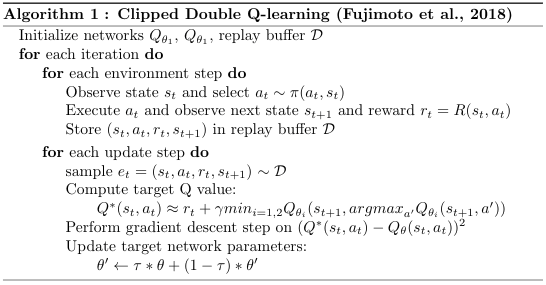
\includegraphics[width=8cm]{alg1_ClippedDDQ_Fujimoto.png}
    \end{center}
    \caption{Clipped Double Q-learning}
    \label{fig:numcomments}
\end{figure}

Clipped Double Q-learning algorithm will be introduced and implemented in the
project to address function approximation errors. Clipped Double Q-learning
algorithm presented by Fujimoto et al. has two major benefits. First, it avoids
overestimation by taking the minimum of the two next-state action values
produced by our two Q networks. When the Q estimate from one is greater than the
other, we reduce it to the minimum, avoiding overestimation. Second, Fujimoto et
al. presents another benefit of this setting: the minimum operator should
provide higher value to states with lower variance estimation error.  This means
that the minimization will lead to a preference for states with low-variance
value estimates, leading to safer policy updates with stable learning targets.

% Import bibligraphy from ref.bib
\bibliography{ref}

\end{document}
